%!TEX root = ..\MainFile.tex
\section{Групповые явления в жизни животных} % (fold)
\label{sec:AnimalFlocking}
\epigraph{Если сто бегунов как один бегут,\\
Это можно назвать так и сяк.\\
У лошадей это будет табун,\\
У рыб это будет косяк.}{Машина Времени}
	\subsection{Методы наблюдения и сбора информации} % (fold)
	\label{sub:ExperimentalMethods}
	Главной сложностью в выполнении экспериментального наблюдения за группой животных или, тем более, насекомых, заключается в трудности отслеживания траекторий отдельных особей. Это связано с тем что рассматриваемые колонии или группы
	\begin{itemize}
		\item  состоят из множества индивидов, которые
		\item выглядят очень похоже
		\item и в основном очень быстро перемещаются
	\end{itemize}
	Кроме того, необходимо учитывать крайнее разнообразие живых организмов, за перемещением которых необходимо наблюдать, поскольку, как уже говорилось во введении, изменение поведения при обьединении в группы наблюдается для широкого разнообразия типоразмеров животных - начиная от бактерий в пробирке \cite{csahok1997,keller1971} и заканчивая китами на океанских просторах \cite{makris2009}.
	Несмотря на совсем неочевидные методы решения этих проблем, изучению стадного поведения (flocking bechavior) на протяжении многих лет посвящалось значительное внимание. Можно заметить что особенно остро (хоть и не в такой формулировке) этот вопрос стоял в 20-е годы XIX столетия на территории Одеской области, которая подвергалась массовым нашествиям саранчи, однако без компьютерного оборудования или без достижения теории ренормализационных групп достичь каких-либо результатов было невозможно.

	Итак, возвращаясь к теме этого пункта, вкратце рассмотрим использующиеся сейчас методы регистрации траекторий индивидов в стаде (стае). Условно, их можно разделить на две неравные группы: в одну отнесем так или иначе методы с использованием визуальных средства (т.е. фото- и видео-камер, в комбинации с различного рода маячками или метками), а в другую сравнительно недавно начавшие применяться методы с использованием GPS-систем. И если применение методов из второй групы не вызывает никаких технических вопросов (кроме, очевидно, закрепления такого рода устройств на исследуемых индивидах), то на методах первой группы следует остановиться подробней.

	Классическим может считаться метод измерение скорости по изображениям частиц \cite{raffel2007}. Обычно он применяется для измерения скорости потока жидкости или газа: в исследуемую среду вводится краситель, состоящий из броуновских частиц, и наблюдая за перемещением этого вещества становится возможным определять линии тока в исследуемой среде. Применимо к самодвижущимся частицам метод успешно был применен Czir\'{o}k и соавторами\cite{csahok1997}, которые при помощи фазово-контрастной микроскопии исследовали групповое движение молекул.

	Когда речь заходит об исследовании стай птиц (стад животных), размер индивидов больше, однако в отличие от бактерий область перемещения слабо ограничена. Тогда движение записывается напрямую на камеру, с тем чтобы в дальнейшем восстановить отдельные траектории. К примеру, в 70-х годах аерофотосьемка использовалась для определения расположения отдельных индивидов во время сбивания африканских буйволов в стадо \cite{sinclair1977}. Однако использования одной камеры для фиксирования перемещений группы рыб или птиц явно недостаточно, поскольку как-то необходимо учитывать расстояние от камеры до особи. Чтобы обойти эту сложность, например, Бекко и соавторы \cite{becco2006} огриничили движение рыб по высоте используя плоский и широкий аквариум.

	Использование нескольких камер для сьемки стай с разных точек в дальнейшем требовало трудоемкой обработки результатов для получения трехмерной картины. Получение стереографических изображений с последующей обработкой позволило определить расстояния между соседними индивидуумами в стаях скворцов и чернозобиков \cite{major1978}. В менее давних исследованиях был обработан метод преобразования фотографий стаи в трехмерные коспьютерные модели, что позволило получить мгновенные снимки положения сотен скворцов в стае \cite{ballerini2008}, однако в задаче восстановление траекторий движения все еще остается поле для исследования.

	По мере развития технологий, стало возможным создать маячки GPS, достаточно маленькие, чтобы их можно было закрепить на животном или птице не мешая ему. К сожалению, с увеличением количества отслеживаемых индивидов возрастает и стоимость исследования. С другой стороны, такого рода устройства обладают ограниченной точностью в определении местоположения. Несмотря на приведенные выше ограничения, были проведены исследования пар \cite{biro2006,nagy2010}, или даже шестерок \cite{dellariccia2008} тренированных голубей.

	Помимо вышесказанного, в настоящее время увеличение точности сонаров и разработка определенной технологии применения, в которой океан выступает в роли акустического волновода позволило использовать их для единовременного наблюдения за огромными количествами рыб на больших территориях океанического шельфа. \cite{makris2006}

	Подводя итоги, можно отметить увеличение роли комьютера в накоплении и обработке экспериментальных данных. Текущая динамика позволяет надеяться что со временем будут получены данные не меньшей точности, чем получаемые во время численных экспериментов по различным моделям.
	% subsection subsection_name (end)

	\subsection{Основные результаты наблюдений} % (fold)
	\label{sub:ExperimentalResults}
	Поскольку экспериментальное наблюдение стадных явлений не является темой данной работы, мы не будем останавливаться подробно результатах полевых или лабораторных исследованиях, тем более что всестороннее освещение этого вопроса дано в работе Вичека~\cite{vicsek2012}. Однако для лучшего понимания распространенности в природе стадных явлений будет приведен краткий обзор наиболее характерных, с нашей точки зрения, работ, сгруппированных по исследуемому материалу. Итак, в разные годы обьектами исследования становились:
	\begin{enumerate}
		\item Внутриклеточные соединения \cite{chowdhury2006,keller1971}
		\item Колонии бактерий \cite{czirok1998,csahok1997}
		\item Насекомые \cite{buhl2006}
		\item Птицы \cite{ballerini2008,selous1931,dellariccia2008,biro2006,major1978,nagy2010}
		\item Рыбы \cite{cambui2012,makris2009,parrish1997}
		\item Млекопитающие, к примеру буйволы \cite{sinclair1977}
	\end{enumerate}
	Особняком в этом ряду стоят наблюдения за океаническим планктоном \cite{seuront2004}, и превышающие по своей численности наблюдения за любым другим типом обьектов наблюдения за поведением групп людей, например \cite{parisi2009,moussaid2011}.%ссылка про транспортные потоки

	Кроме того, в совершенно отдельную группу необходимо выделить лабораторные эксперименты, проводимые с неживыми обьектами - нематической жидкостью, колеблющимися металлическими стержнями, нано частицами в жидкости, микро роботами и тому подобным. \cite{schaller2010,turgut2008,blair2003}

	Теперь, приведем основные результаты, полученные в ходе наблюдений. Для начала, наобходимо четко разделять работы в которых исследования велись на плоскости (все кроме указанных далее), и в которых наблюдения велись в трехмерном пространстве \cite{cullen1965,ballerini2008,major1978,makris2009}. Хотя, как выяснилось, для рыб такое разделение не вполне необходимо. Но обо всем по порядку.

	Главный вывод, который в общем-то и не нуждается в подтверждении - это то, что существует отдельный класс перемещений группы индивидов как целого, и при этом перемещения отдельных индивидов оказываются упорядочены. То есть, при определенных условиях (чаще всего рассматривается различная плотность на единицу площади, или обеспеченность ресурсами в широком смысле слова) происходит спонтанное нарушение симметрии, и хаотическое движение сменяется упорядоченным. Как уже говорилось, это наблюдается на всех масштабах природы, и более того - совершенно не обязательно при этом прямое (визуальное или тактильное) взаимодействие между особями, и бывает достаточно опосредствованного взаимодействия через среду обитания \cite[с. 119]{vicsek2012}. %добавить информацию про молекулы, перекидывающие взаимодействие через жидкость в которой они живут
	Следующее наблюдение на которое указывают многие авторы - при нарушении симметрии возникает и дальний порядок связи, к примеру, рыбы могут изменять общее направление движения практически мгновенно \cite{cambui2012}, а птицы так-же быстро принимать решения о посадке. \cite{lukeman2010,major1978}.

	Но более того, самым удивительным явлется то, что у всех живых существ и неживых предметов, при движении которых проявляются стадные явления, качественный характер этих явления практически одинаков. %(Не считая сугубо трехмерных формаций, которые образуются в стаях птиц, однако и там можно выделить правильный ``параметр порядка'').
	\begin{figure}
        \centering
        \begin{subfigure}{.4\columnwidth}
                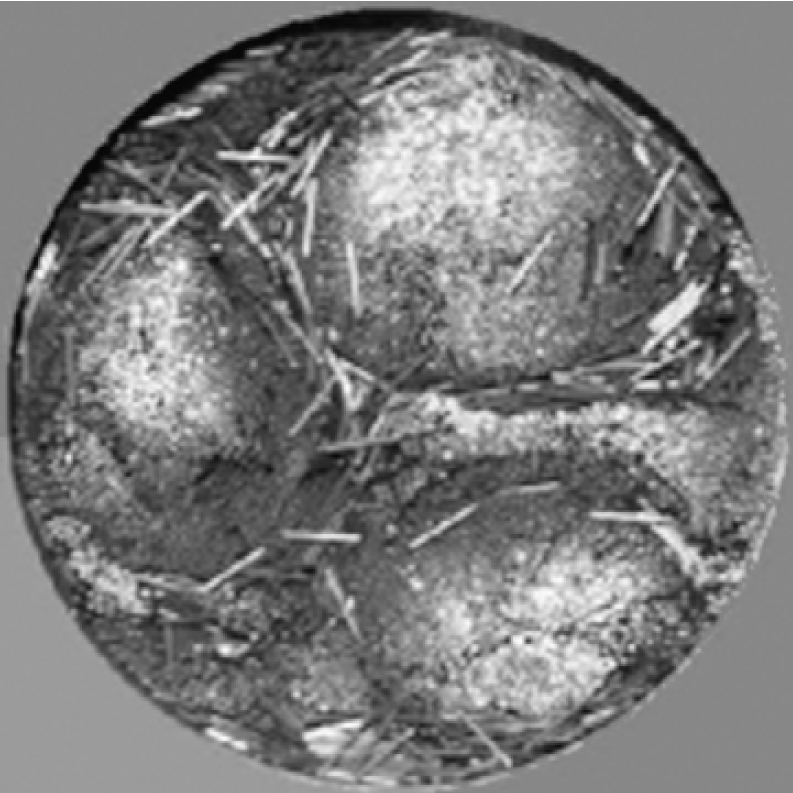
\includegraphics[width=\columnwidth]{Fig4_CollectiveMotion}
                \caption{A nematics}
                \label{fig:CollMot:nematics}
        \end{subfigure}%
        ~ %add desired spacing between images, e. g. ~, \quad, \qquad, \hfill etc.
          %(or a blank line to force the subfigure onto a new line)
        \begin{subfigure}{.4\columnwidth}
                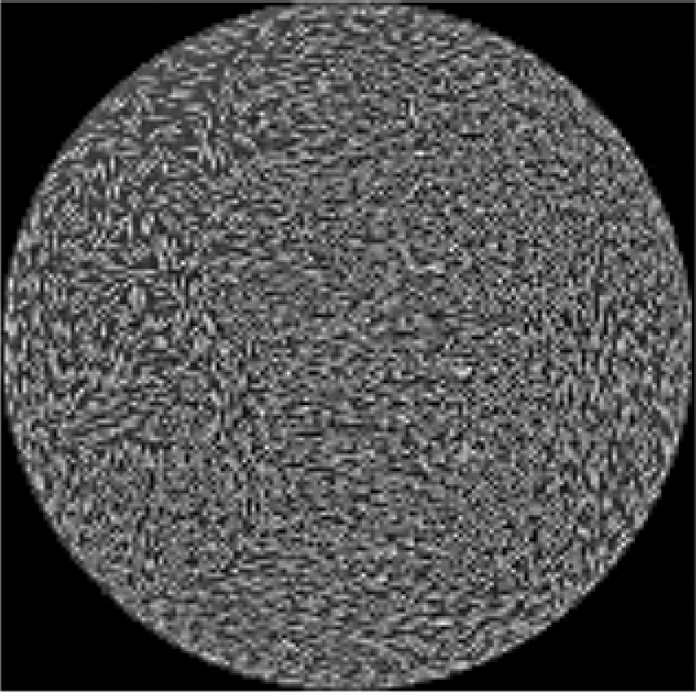
\includegraphics[width=\columnwidth]{Fig6_CollectiveMotion}
                \caption{A rods on wibe}
                \label{fig:CollMot:rods}
        \end{subfigure}
        \caption{Упорядочивание неживых обьектов}
        \label{fig:CollMot:NonLiving}
    \end{figure}
        ~ %add desired spacing between images, e. g. ~, \quad, \qquad, \hfill etc.
          %(or a blank line to force the subfigure onto a new line)
    \begin{figure}
    	\centering
        \begin{subfigure}{0.3\textwidth}
                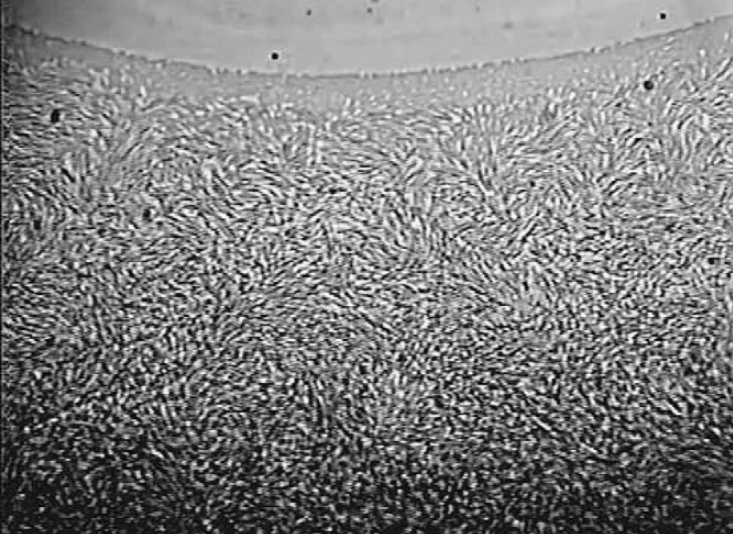
\includegraphics[width=\textwidth]{Fig11_CollectiveMotion}
                \caption{A bacteria 1}
                \label{fig:CollMot:bacteria}
        \end{subfigure}
        \begin{subfigure}{0.5\textwidth}
                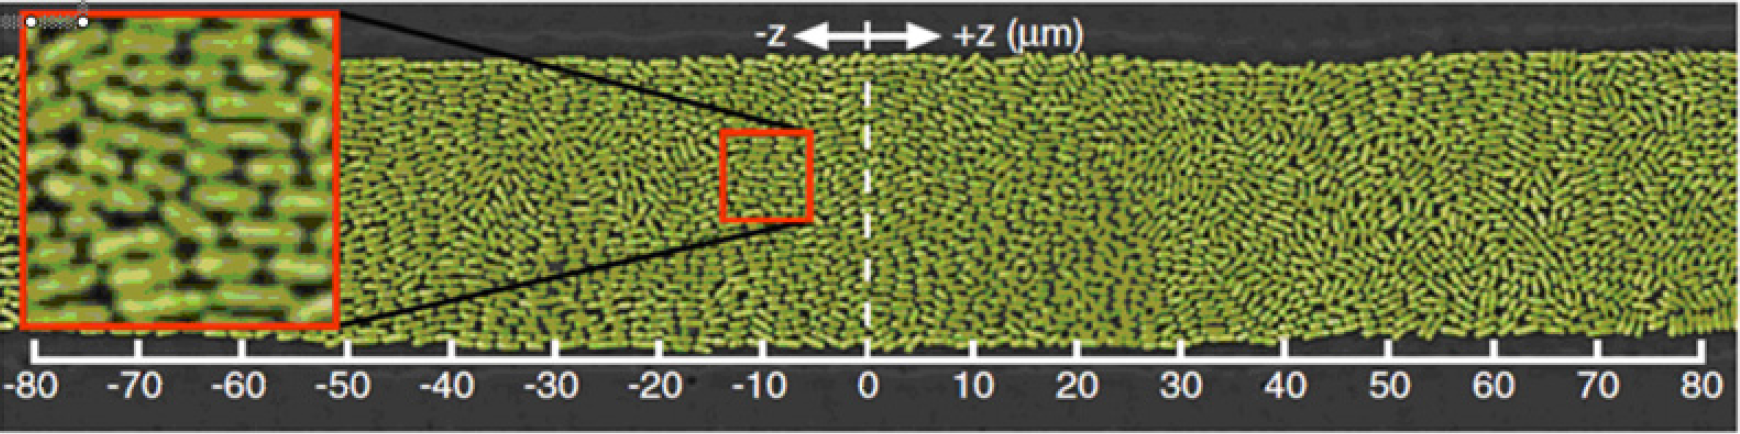
\includegraphics[width=\textwidth]{Fig15_CollectiveMotion_part}
                \caption{A moleculae}
                \label{fig:CollMot:moleculae}
        \end{subfigure}
        \caption{Микроскопические проявления групповой динамики}
        \label{fig:CollMot:microscpoic}
    \end{figure}
    \begin{figure}
    	\centering
        \begin{subfigure}{0.4\textwidth}
                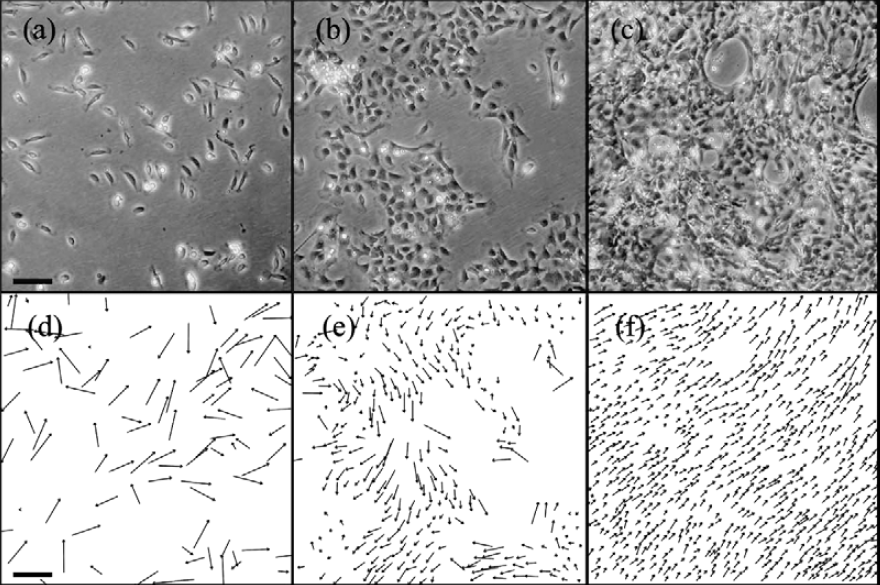
\includegraphics[width=\textwidth]{Fig17_CollectiveMotion}
                \caption{A fishes}
                \label{fig:CollMot:fishes}
        \end{subfigure}
        \begin{subfigure}{0.4\textwidth}
                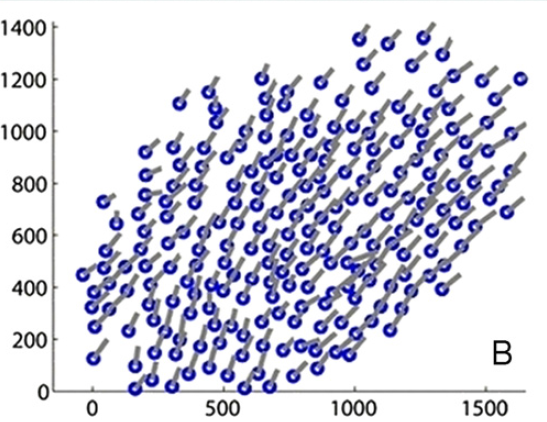
\includegraphics[width=\textwidth]{Fig29_CollectiveMotion_part}
                \caption{A ducks}
                \label{fig:CollMot:ducks}
        \end{subfigure}
        \caption{Макроскопические проявления группового движения}\label{fig:CollMot:macroscopic}
	\end{figure}

	Наглядно это можно рассмотреть на рис. \ref{fig:CollMot:NonLiving}, \ref{fig:CollMot:microscpoic}, \ref{fig:CollMot:macroscopic}. Особенностью всех представленных на изображениях обьединений является то, что они расположены на плоскости. И как мы видим, возникает два типа упорядоченностей, иногда (как на рис. \ref{fig:CollMot:nematics}) проявляющихся единовременно: это упорядоченное движение в спонтанно выбранном направлении, или упорядоченное обращение вокруг некоторого центра. Видно также, что для совершенно, казалось бы, различных обьектов групповое поведение является очень схожим.

	Что же касается перемещений, не ограниченных в двух плоскостях, то нам хотелось бы заострить внимание на трех моментах. 

	Во-первых, в обьемном пространстве также наблюдаются все вышеперечисленные упорядоченные перемещения: птицы сбиваются в стаю и летят в выбранном направлении \cite{dellariccia2008}, насекомые кружат вокруг улья \cite{buhl2006} и т.п.

	\begin{wrapfigure}{r}{0.5\textwidth}
	  \vspace{-20pt}
	  \begin{center}
	    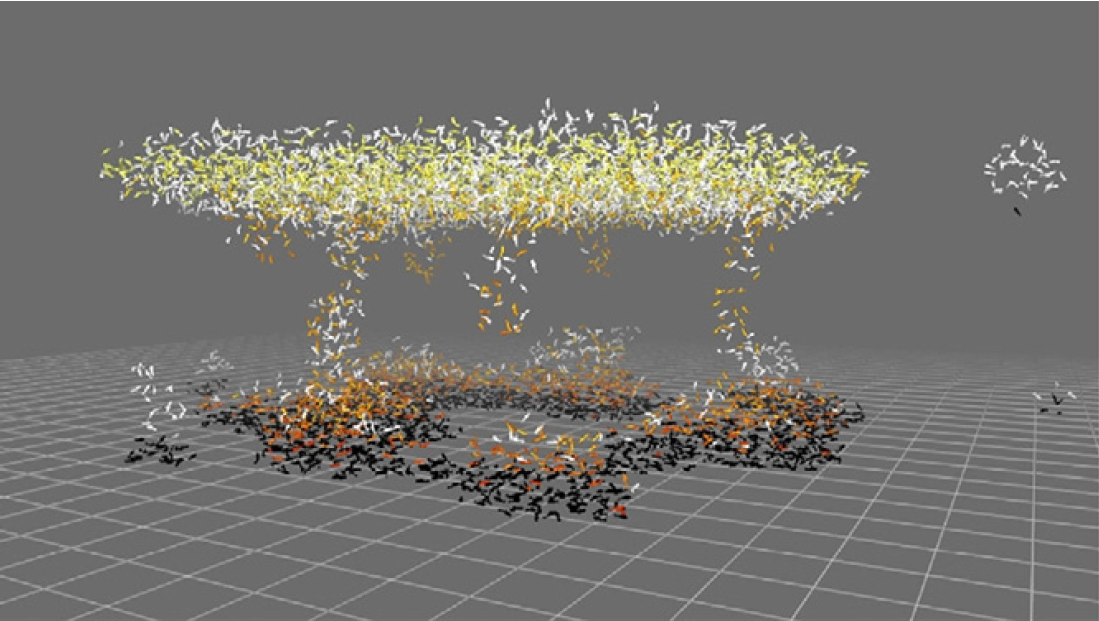
\includegraphics[width=0.48\textwidth]{Fig57_CollectiveMotion}
	  \end{center}
	  \vspace{-20pt}
	  \caption{Расслоение косяка рыб}
	  \label{fig:FishSplitting}
	  \vspace{-10pt}
	\end{wrapfigure}

	Во-вторых, и это является особенностью косяков рыб, возможно расслоение трехмерной группы на более плоские подгруппы, с наличием соединяющих (цилиндрических) столбов. Предполагается, что это это связано с ``мотивацией'', например, молодая стерлядь во время нереста предпочитает подниматься выше, а более старая опускается вниз. \cite{axelsen2000} При этом наблюдаются структуры как изображенные на рис. \ref{fig:FishSplitting}

    \begin{figure}
    	\centering
        \begin{subfigure}{0.4\textwidth}
                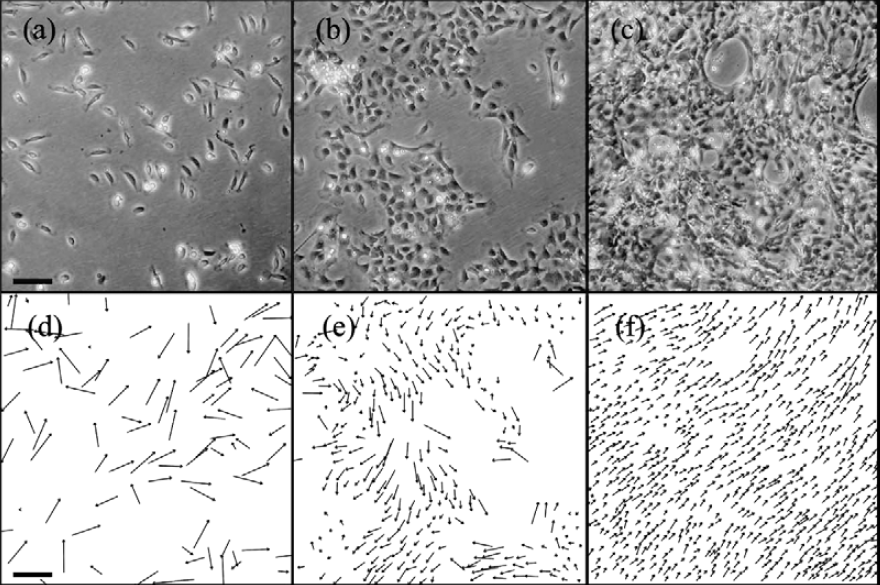
\includegraphics[width=\textwidth]{Fig17_CollectiveMotion}
                \caption{A fishes}
                \label{fig:CollMot:Birds}
        \end{subfigure}
        \begin{subfigure}{0.4\textwidth}
                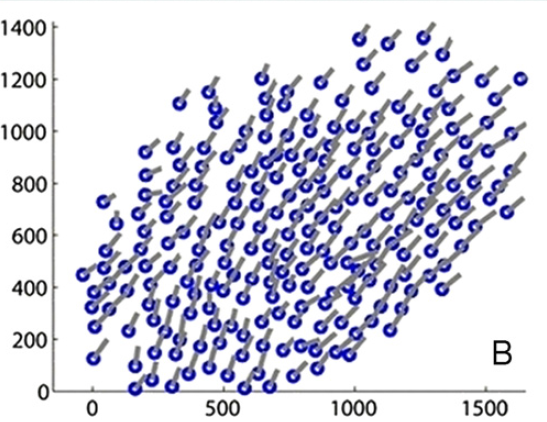
\includegraphics[width=\textwidth]{Fig29_CollectiveMotion_part}
                \caption{A ducks}
                \label{fig:CollMot:Plancton}
        \end{subfigure}
        \caption{Макроскопические проявления группового движения []}\label{fig:CollMot:Volumetric}
	\end{figure}

	И в третьих, поскольку основное внимание при наблюдениях в трехмерном пространстве уделялось птицам и рыбам, групповая динамика которых хоть и обладает большим количеством подобных черт, все-же разнятся в том что стаи птиц не расслаиваются по высоте, тем более ярко проявляется аналогия между пространственными формированиями птиц и морского планктона []%уточнить!!!!
	% subsection основные_результаты_наблюдений_за_системами_демонстрирующими_группувую_динамику (end)

% section групповые_явления_в_жизни_животных (end)